
% part 2
\section{Медленная поэзия и апокалипсис\label{sec:part2}}


    На этот раз мы запачкаем наши руки и напишем некоторый код. Но сначала - 
некоторые предположения.


\subsection{Предположения о навыках}


    Предполагается, что вы имеете некоторые навыки написания 
синхронных программ на Python'е и немного знаете о 
сокетном программировании на Python'е. Если вы никогда раньше не 
использовали сокеты, вы можете почитать 
\href{http://docs.python.org/library/socket.html#module-socket}{документацию о Python-модуле socket}, 
особенно примеры ближе к концу. Если вы никогда раньше не 
использовали Python, то все остальное вам, вероятно, покажется странным.  


\subsection{Предположения о компьютере}


    Примеры разрабатывались и отлаживались на Linux'е. 
Возможно, что код работает 
под другие Unix подобные системы (Mac OSX или FreeBSD).


Далее предполагается, что вы установили относительно свежые  
версии 
\href{http://python.org/download}{Python} и 
\href{http://twistedmatrix.com/trac/wiki/Downloads}{Twisted}. 
Примеры разрабатывались с использованием 
Python 2.5 и Twisted 8.2.0.


Вы можете запускать все примеры на одном компьютере или 
сконфигурировать их для запуска по сети на 
нескольких машинах. Но для изучения основных механизмов 
асинхронного программирования использование одной 
машины предпотчтительнее.


Код с примерами доступен ввиде  
\href{http://github.com/jdavisp3/twisted-intro/zipball/master}{zip} или 
\href{http://github.com/jdavisp3/twisted-intro/tarball/master}{tar} файла, или как 
\href{http://github.com/jdavisp3/twisted-intro/tree/master}{git репозиторий}. 
Если вы можете использовать git 
или другую систему контроля версий, которая может читать 
git репозиторий, то рекомендуется использовать этот метод, 
так как примеры время от времени обновляются, и в этом случае 
обновление будет осуществляться гораздо проще. Репозиторий 
помимо всего прочего  
включает исходники рисунков в формате SVG. 
Клонировать репозиторий можно следующим образом: 

\begin{scriptsize}\begin{verbatim}
git clone git://github.com/jdavisp3/twisted-intro.git
\end{verbatim}\end{scriptsize}

И последнее предположение: наличие нескольких консолей, 
открытых в директории с примерами (в одной из них предполагается 
открытым файл README).


\subsection{Медленная поэзия}


    Хотя процессоры намного быстрее, чем сети, 
а большинство сетей все же намного быстрее, чем мозг, 
или по меньшей мере быстрее, чем скорость движения 
глаз. Сложно получить заметную задержку в сети, особенно, в случае 
одной машины и байтов, проносящихся со свистом на  
\href{http://en.wikipedia.org/wiki/Loopback}{loopback интерфейсе}. 
То что нам нужно - медленный сервер, 
с искуственными задержками, которые мы можем менять для 
изучения их воздействия. Поскольку серверы должны что-то 
обслуживать, то наш сервер будет обслуживать поэзию. 
В исходниках примеров находится директория poetry с поэзией авторов 
\href{http://en.wikipedia.org/wiki/Donne}{John Donne},
\href{http://en.wikipedia.org/wiki/Yeats}{W.B. Yeats}, 
\href{http://en.wikipedia.org/wiki/Poe}{Edgar Allen Poe}. 
Конечно же, вы можете использовать свои собственные поэмы. 


Медленный поэтический сервер реализован в 
\href{http://github.com/jdavisp3/twisted-intro/blob/master/blocking-server/slowpoetry.py}{blocking-server/slowpoetry.py}. 
Вы можете запустить пример сервера следующим образом:

\begin{scriptsize}\begin{verbatim}
python blocking-server/slowpoetry.py poetry/ecstasy.txt
\end{verbatim}\end{scriptsize}


Эта команда запустит блокирующий сервер с 
поэмой “Ecstasy” John Donne. Пойдем дальше и посмотрим на 
исходный код блокирующего сервера. Как можно заметить, в 
коде не используется Twisted, только основные сокетные 
операции. Сервер отправляет ограниченное количество 
байт за раз, с фиксированной временной задержкой между ними. 
По умолчанию, сервер отправляет 10 байт каждые 0.1 секунды, 
но вы можете поменять эти параметры с помощью опций 
командной строки \textit{\symbol{45}\symbol{45}num-bytes} и 
\textit{\symbol{45}\symbol{45}delay}. Например, чтобы 
отправлять 50 байт каждые 5 секунд, нужно запустить: 

\begin{scriptsize}\begin{verbatim}
python blocking-server/slowpoetry.py --num-bytes 50 --delay 5 poetry/ecstasy.txt
\end{verbatim}\end{scriptsize}


Когда сервер запускается, он печатает номер порта, который он 
слушает. По умолчанию, это первый доступный случайный порт на вашей машине. 
Запуская сервер с различными настройками, может понадобится использовать 
тот же порт, что и до этого, для того, чтобы не нужно было 
перенастраивать клиент. Вы можете задать определенный порт следующим образом:

\begin{scriptsize}\begin{verbatim}
python blocking-server/slowpoetry.py --port 10000 poetry/ecstasy.txt
\end{verbatim}\end{scriptsize}

Если у вас есть программа 
\href{http://netcat.sourceforge.net/}{netcat} (или nc), можно протестировать 
запущенный сервер следующим образом:

\begin{scriptsize}\begin{verbatim}
netcat localhost 10000
\end{verbatim}\end{scriptsize}


При запущенном сервере вы увидите медленно ползущую 
вниз по экрану поэму. Экстаз! Вы также заметите, что сервер 
печатает строки с количеством отосланных байт. Сразу после того, как 
поэма была отослана, сервер закрывает соединение.


По умолчанию, сервер слушает только локальный "loopback" 
интерфейс. Если вы хотите получить доступ к серверу с 
другой машины, вы можете задать сетевой интерфейс через 
опцию --iface.


Сервер не только медленно отправляет поэму, по коду видно, что 
во время отправления сервером поэмы одному клиенту, другие 
клиенты должны ожидать окончания скачивания поэмы первым клиентом 
до того, как другие смогут получить хотя бы первую строку. 
Это реально медленный сервер и не особо полезен, кроме как 
в обучающих целях. 


С другой стороны, если большинство пемиссемистичных 
людей из 
\href{http://www.peakoil.net/}{Peak Oil} правы, и нашему миру грозит 
глобальный энергетический и социальный кризис, то, однажды, 
низкопропускной и маломощный сервер может стать именно тем, что нам 
нужно. Представьте, что после длительного дня забот о ваших 
садах, производстве собственной одежды, обслуживания 
Центрального Организационного Комитета Вашей комунны, борьбы 
с радиокативными зомби, бродящими по пост-апокалиптическим 
пустошам, вы сможете покрутить ваш генератор и скачать 
несколько строк высокой культуры из исчезнувшей цивилизации. 
Вот тогда наш сервер реально вcтупит в свои права. 


\subsection{Блокирующий клиент}


    Также в исходных кодах можно найти пример блокирующего 
клиента, который скачивает поэмы из серверов одну за 
другой. Давайте дадим нашему клиенту три задачи для 
выполнения так, как это изображено на рисунке \ref{fig:sync}. 
Сначала мы запустим три сервера, обслуживающих три 
различных поэмы:

\begin{scriptsize}\begin{verbatim}
python blocking-server/slowpoetry.py --port 10000 poetry/ecstasy.txt --num-bytes 30
python blocking-server/slowpoetry.py --port 10001 poetry/fascination.txt
python blocking-server/slowpoetry.py --port 10002 poetry/science.txt
\end{verbatim}\end{scriptsize}


Вы можете выбрать другие номера портов, если те, 
что выбраны выше, уже используются в вашей системе. 
Заметьте, что первый сервер использует chunk'и по 
30 байт, вместо 10, что установлены по умолчанию, 
поскольку поэма, которую он обслуживает  примерно 
в три раза длиньше остальных. При таких настройках 
скачивание каждой из них должно завершаться 
приблизительно в одно и тоже время.


Теперь мы можем запустить блокирующий клиент из 
\href{http://github.com/jdavisp3/twisted-intro/blob/master/blocking-client/get-poetry.py}{blocking-client/get-poetry.py}, 
для того, чтобы скачать немного поэзии. Запустите клиент следующим образом:

\begin{scriptsize}\begin{verbatim}
python blocking-client/get-poetry.py 10000 10001 10002
\end{verbatim}\end{scriptsize}


Вы также можете поменять номера портов, если сервера 
слушают на других портах. Поскольку мы имеем дело с 
блокирующим клиентом, то он будет скачивать одну поэму 
из каждого порта по очереди, ожидая пока поэма будет 
полностью получена до того, как начать скачивать 
следующую поэму. Вместо печати поэм, блокирующий клиент 
выводит нечто вроде: 

\begin{scriptsize}\begin{verbatim}
Task 1: get poetry from: 127.0.0.1:10000
Task 1: got 3003 bytes of poetry from 127.0.0.1:10000 in 0:00:10.126361
Task 2: get poetry from: 127.0.0.1:10001
Task 2: got 623 bytes of poetry from 127.0.0.1:10001 in 0:00:06.321777
Task 3: get poetry from: 127.0.0.1:10002
Task 3: got 653 bytes of poetry from 127.0.0.1:10002 in 0:00:06.617523
Got 3 poems in 0:00:23.065661
\end{verbatim}\end{scriptsize}

Это очень похоже на текстовую версию рисунка \ref{fig:sync}, где 
каждая задача качает одну поэму. В вашем выводе времена скачиваний  
могут немного отличаться. Ими можно вариьровать через параметр сервера 
\textit{\symbol{45}\symbol{45}delay}. 
Попробуйте поменять его и увидеть как меняется время скачивания.


Теперь можно посмотреть на исходный код блокирующего сервера и 
клиента и отметить места в коде, где они блокируются при 
отправлении или получении сетевых данных.


\subsection{Асинхронный клиент}


    Давайте теперь посмотрим на реализацию простого 
асинхронного клиента, написанного без ипользования 
Twisted. Сначала давайте его запустим. Запустите три сервера, 
как мы это делали выше. 
Если они все еще запущены, то мы можем снова их 
использовать. Теперь запустим асинхронный клиент, 
расположенный в 
\href{http://github.com/jdavisp3/twisted-intro/blob/master/async-client/get-poetry.py}{async-client/get-poetry.py},  
как написано ниже:

\begin{scriptsize}\begin{verbatim}
python async-client/get-poetry.py 10000 10001 10002
\end{verbatim}\end{scriptsize}


В результате получится примерно такой вывод:

\begin{scriptsize}\begin{verbatim}
Task 1: got 30 bytes of poetry from 127.0.0.1:10000
Task 2: got 10 bytes of poetry from 127.0.0.1:10001
Task 3: got 10 bytes of poetry from 127.0.0.1:10002
Task 1: got 30 bytes of poetry from 127.0.0.1:10000
Task 2: got 10 bytes of poetry from 127.0.0.1:10001
...
Task 1: 3003 bytes of poetry
Task 2: 623 bytes of poetry
Task 3: 653 bytes of poetry
Got 3 poems in 0:00:10.133169
\end{verbatim}\end{scriptsize}

На этот раз вывод намного длиньше, поскольку клиент выводит 
строку после каждого скачивания порции данных с любого сервера. 
Сервера, как и раньше, понемногу отдают поэзию. 
Заметьте, что выполнение отдельных задач чередуется, как это изображено на 
рисунке \ref{fig:async}.


Попробуйте поменять опцию \textit{\symbol{45}\symbol{45}delay} 
для серверов (например, сделать 
один сервер медленнее, чем остальные) для того, чтобы увидеть 
как асинхронный клиент автоматически "подстроится" под скорость 
медленных серверов, в тоже время успевая за быстрыми серверами. 
Это асинхронность в действии. 


Также заметьте, что при найстройках сервера, которые были установлены 
выше, асинхронный 
клиент завершается примерно за 10 секунд, в то время как 
синхронному клиенту требуется примерно 23 секунды для получения 
всех поэм. Теперь вернемся к отличиям между рисунками \ref{fig:async} и 
\ref{fig:block}. Тратя меньше времени на блокирование, наш 
асинхронный клиент может скачать все поэмы за более короткий промежуток 
времени, поскольку он переключается между всеми медленными серверами.


Технически, наш асинхронный клиент выполняет блокирующую операцию: 
он пишет в стандартный вывод, используя оператор print! Это не 
является проблемой в нашем случае. На локальной машине с 
терминальным shell'ом, готовым принять вывод, оператор print 
не будет реально блокироваться и будет выволняться досточно быстро 
по сравнению с нашими медленными серверами. Но, если бы мы захотели, 
чтобы наша программа была частью pipeline и все еще выполнялась 
асинхронно, нам нужно было бы использовать асинхронный ввод-вывод 
для стандартного ввода и вывода. Twisted имеет модули, реализующие это, 
но для простоты, мы будем использовать 
оператор print, даже в программах, написанных с использованием Twisted.


\subsection{Пристальный взгляд}


    Теперь давайте посмотрим на исходный код асинхронного клиента. 
Отметим основные отличия между ним и синхронным клиентом:

\begin{enumerate}
\item Вместо соединения только с одним сервером в один момент времени  
асинхронный клиент соединяется со всеми серверами одновременно.

\item Сокетные объекты, использованные для соединения, устанавливаются в неблокирующее 
состояние с использованием вызова setblocking(0).

\item Используется метод select из модуля 
\href{http://docs.python.org/library/select.html#module-select}{select} для ожидания (блокирования) 
до того момента, когда хотя бы один из сокетов готов отдать некоторую 
порцию данных.

\item При чтении данных из серверов мы читаем по максимуму до 
момента блокирования сокета, затем переходим к чтению данных 
из следующего имеющегося готового к чтению сокета. 
\end{enumerate}


Ядром асинхронного клиента является внешний цикл в 
функции get\_poetry. Этот цикл можно разбить на 
несколько шагов:

\begin{enumerate}
\item Ожидание (блокирование) всех открытых сокетов с использованием select'а, 
до тех пор пока один или более сокетов будут иметь данные для считывания. 
\item Для каждого сокета с готовыми для считывания данными, прочитать их, но только 
в количестве, доступном на данный момент, чтобы избежать 
\href{http://en.wikipedia.org/wiki/Asynchronous\_I/O}{блокирования}.
\item Повторять шаги выше до момента закрытия сокетов.
\end{enumerate}


Синхронный клиент также имеет цикл (в функции main), но 
при каждой итерации цикла в синхронном клиенте скачивается полностью 
одна поэма. В то время как при каждой итерации асинхронного 
клиента скачиваются куски поэм. И мы не знаем, 
над какими из них мы будем работать в данной итерации, или 
сколько данных мы получим от каждой из них. Все это зависит от 
относительных скоростей серверов и состояния сети. Мы только 
позволяем select'у сообщать нам о том, какие сокеты готовы на чтение, 
и читаем столько данных, сколько можем из каждого сокета, не блокируясь.


Если бы синхронный клиент соединялся бы 
с фиксированным количеством серверов (скажем тремя), 
нам бы совершенно не понадобился внешний цикл, поскольку 
можно было бы последовательно вызвать три раза 
функцию get\_poetry. Но асинхронный клиент не может 
обходиться без внешнего цикла, поскольку нужно одновременно 
опрашивать все сокеты и обрабатывать столько 
данных, сколько было доставлено за заданную итерацию. 


Использование подобного цикла, ожидающего событий и 
управляющего ими, является общепринятым, и известно как 
\href{http://en.wikipedia.org/wiki/Reactor\_pattern}{шаблон проектирования reactor}. 
Изложенное выше проиллюстрировано на рисунке \ref{fig:reactor-1}:

% fig5
\begin{figure}[h]
\begin{center}
    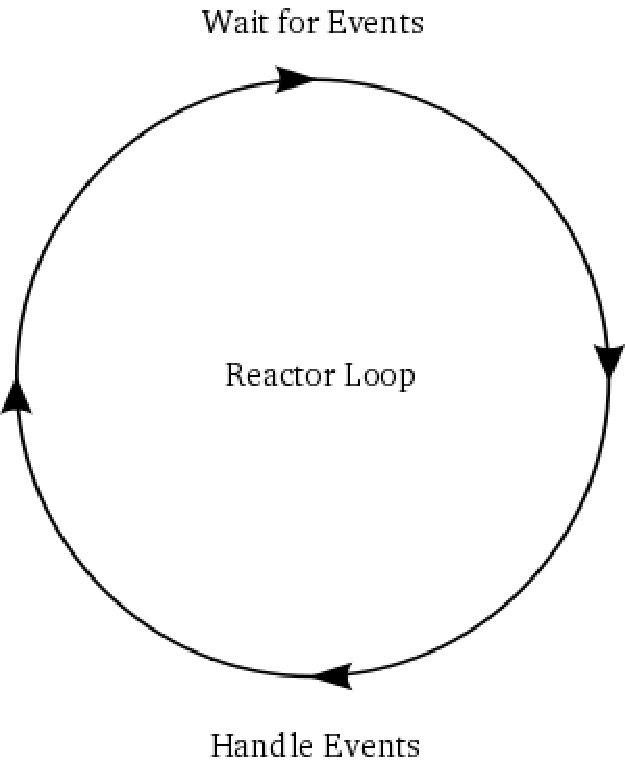
\includegraphics[width=0.3\textwidth]{images/reactor-1.pdf}
\end{center}
    \caption{Цикл reactor'а\label{fig:reactor-1}}
\end{figure}

\eject

Цикл является “reactor'ным”, поскольку он ожидает событий 
и затем реагирует на них. По этой причине, такой цикл 
известен также как "event loop". Поскольку реактивные 
системы зачастую ожидают ввода-вывода, такие циклы зачастую 
называют 
\href{http://en.wikipedia.org/wiki/Asynchronous\_I/O#Select.28.2Fpoll.29\_loops}{select циклы}, 
поскольку вызов select используется для ожидания ввода-вывода. 
Таким образом в select циклах, "событием" является момент, когда 
сокет становится доступным на чтение или запись. Надо отметить, что 
select - не единственный способ ожидания ввода-вывода, это один 
из самых старых (поэтому широко доступных) методов. Существует несколько 
более новых API, доступных на различных операционных системах, 
которые делают те же вещи, что и select, но имеют лучшую 
производительность. Но, невзирая на производительность, они все делают 
одно и тоже: берут множество сокетов (реально файловых дескрипторов) и 
блокируются до тех пор, пока один или более из них не станут готовы для 
операций ввода-вывода.  


Нужно отметить, что можно использовать select и его 
товарищей для простой проверки на готовность множества 
файловых дескрипторов для операций ввода-вывода без 
блокирования. Это свойство позволяет реагирующей системе (reactive system) 
выполнять что-либо, не являющееся вводом-выводом, 
внутри цикла. Но в реагирующих системах в основном вся работа 
связана с вводом-выводом, таким образом блокирование на 
всех файловых дескрипторах сохранит ресурсы процессора.


Говоря точно, цикл в нашем асинхронном клиенте не соответсвует 
шаблону проектирования reactor, поскольку логика в цикле не 
реализована отдельно от основной логики, которая является 
специфичной для поэтических серверов. Они просто перемешаны 
друг с другом. Реальная реализация шаблона проектирования reactor 
реализовывала бы цикл как отдельную абстракцию, способную:

\begin{enumerate}

\item Принимать множество файловых дескрипторов для выполнения 
операций ввода-вывода.

\item Циклически сообщать о том, когда любой из файловых дескриторов 
готов на чтение или запись. 

\end{enumerate}


А реально хорошая реализация шаблона проектирования reactor 
делала бы:

\begin{enumerate}

%   1. Handle all the weird corner cases that crop up on different systems.
\item Управление всеми проблемными случаями, которые происходят на 
различных системах.

%   2. Provide lots of nice abstractions to help you use the reactor with the least amount of effort.
\item Обеспечение множеством абстракций, помогающих использовать 
reactor с минимальными усилиями.

%   3. Provide implementations of public protocols that you can use out of the box.
\item Предоставление реализаций основных протоколов, которые можно тут же использовать.

\end{enumerate}

В целом, Twisted - это устойчивая, кросс-платформенная 
реализация шаблона проектирования reactor со 
множественными дополнениями. И в следующей главе мы 
начнем писать простые программы с использованием Twisted, 
так что сейчас мы движемся напрямую к получению поэзии со вкусом Twisted!


\subsection{Упражнения}

\begin{enumerate}

\item Проделайте несколько экспериментов с блокирующей 
и асинхронной версиями клиента, меняя количество и настройки 
поэтических серверов.

\item Может ли асинхронный клиент предоставить функцию get\_poetry, 
которая возвращала бы текст поэмы? Почему нет?

\item Если бы вы хотели реализовать функцию get\_poetry в 
асинхронном клиенте аналогичную синхронной версии, как бы 
это могло работать? Какие аргументы и возвращаемые значения  
были бы в этом случае?

\end{enumerate}



